\documentclass[../../main.tex]{subfiles}
\graphicspath{{../../image/}{../../figure/}}
\begin{document}

\section{真正非线性失效时}\label{section:ch11-真正非线性失效时}

如本章前几节所示, 带凸通量的标量守恒律可容许 $BV$ 解中的跳跃间断必为压缩激波。正是这一性质诱导出极值后向特征线的特殊结构, 记录在\cref{theorem:ch11-11-3}中, 它对于将 $BV$ 解的结构化繁为简起关键作用。相反, 当通量具有拐点时, 接触间断的出现引起相当大的复杂化。广义特征线工具仍然有效, 但分析变得相当繁琐。

本节讨论标量守恒律的最简单情形:
\begin{align}
\partial_t u(x,t)+\partial_x f(u(x,t))=0,\label{align:ch11-11-12-1}
\end{align}
其中光滑通量 $f$ 在原点有单一拐点,
\begin{align}
u f''(u)<0,\qquad u\neq0,\label{align:ch11-11-12-2}
\end{align}
非退化, 阶为某偶数 $m$。为方便起见, 标度 $u$ 使
\begin{align}
f^{(j)}(0)=0,\quad j=0,1,\ldots,m,\qquad f^{(m+1)}(0)=-m!.\label{align:ch11-11-12-3}
\end{align}

读者应注意, 此例仅展示真正非线性缺失时可能遇到的部分复杂性。首先, 在假设\eqref{align:ch11-11-12-2}下, Oleinik $E$-条件仅允许左接触间断, 右接触间断不可容许。此外, 中心稀疏波不能由波相互作用产生。不过, 非中心稀疏简单波可自左接触间断向外辐射。

设 $u$ 是\eqref{align:ch11-11-12-1}在 $(-\infty,\infty)\times[0,\infty)$ 上的解, 初值 $u_0$ 取值于区间 $[-\bar u,\bar u]$ 且在 $(-\infty,\infty)$ 上局部有界变差。归一化 $u_0(\cdot)$ 与 $u(\cdot,t)$ 使其左连续。

时间区间 $[\sigma,\tau]\subset[0,\infty)$ 上的 Lipschitz 曲线 $\xi(\cdot)$ 称为与解 $u$ 关联的广义特征线, 若\eqref{align:ch11-11-1-3}对几乎所有 $t\in[\sigma,\tau]$ 成立。

解 $u$ 满足可容许性条件
\begin{align}
\partial_t\eta(u(x,t))+\partial_x q(u(x,t))\leqslant0,\label{align:ch11-11-12-4}
\end{align}
对任意凸函数 $\eta$ (充当熵), 熵流 $q$ 由 $q'(u)=\eta'(u)f'(u)$ 确定。若 $\xi(\cdot)$ 是定义在 $[\sigma,\tau]$ 上的特征线, 由\eqref{align:ch11-11-1-3}与\eqref{align:ch11-11-12-4}易得
\begin{align}
q(u(\xi(t)+,t))-q(u(\xi(t),t))-\dot{\xi}(t)[\eta(u(\xi(t)+,t))-\eta(u(\xi(t),t))]\leqslant0,\label{align:ch11-11-12-5}
\end{align}
对几乎所有 $t\in[\sigma,\tau]$。回忆\cref{chapter:ch08-容许激波}, \eqref{align:ch11-11-12-5}蕴含 Oleinik $E$-条件\cref{chapter:ch08-容许激波}对几乎所有 $t\in[\sigma,\tau]$ 且 $u(\xi(t)+,t)\neq u(\xi(t),t)$ 成立。


\begin{figure}[htbp]
\centering
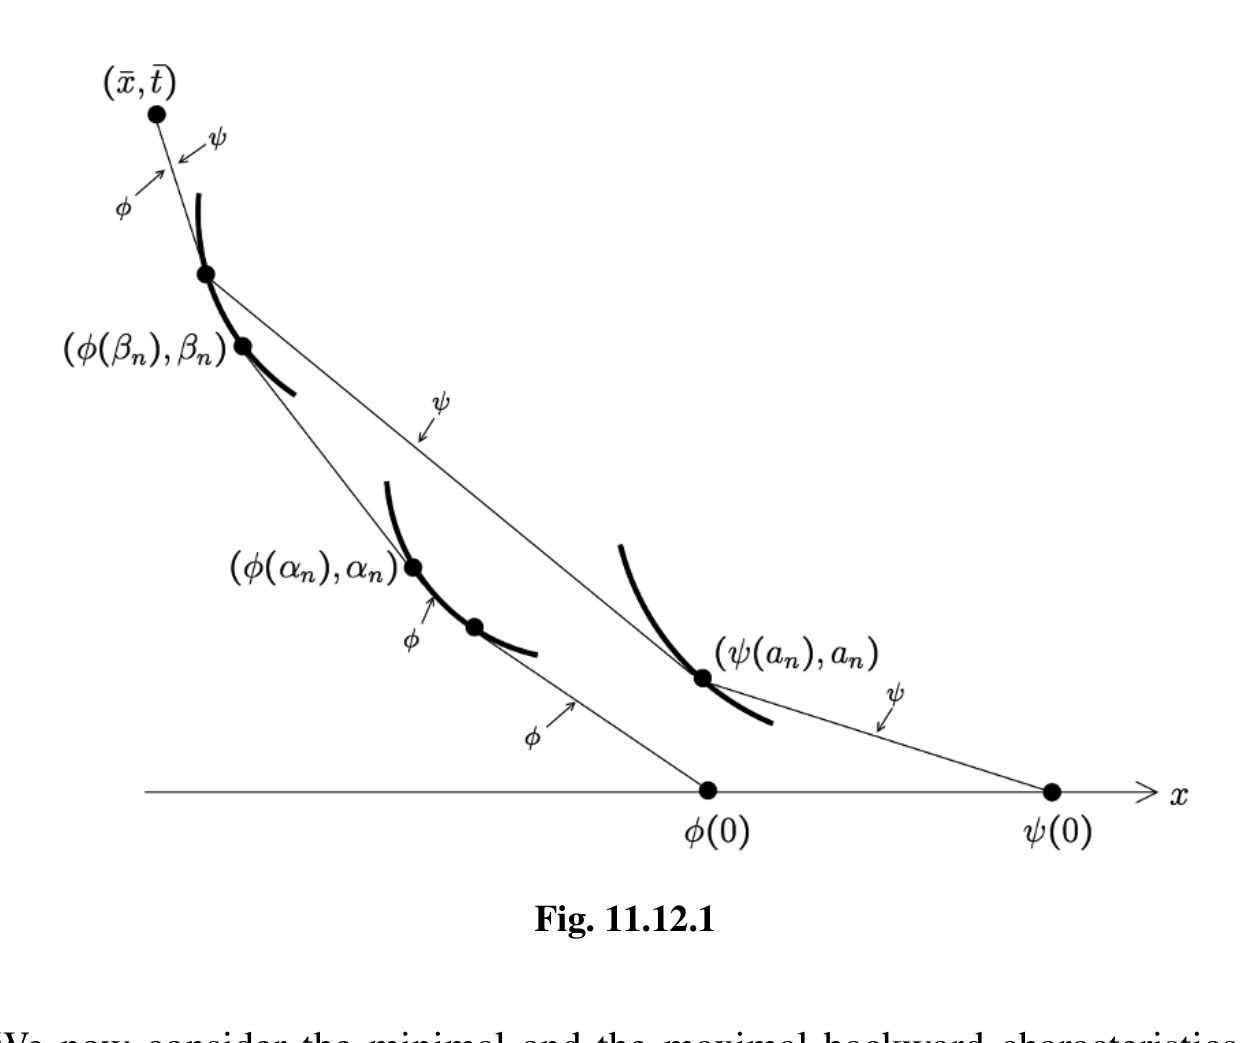
\includegraphics[width=0.75\textwidth]{ch11-fig12-1.png}
\caption{极值后向特征线 $\phi(\cdot)$ 与 $\psi(\cdot)$ 的结构。}
\label{figure:ch11-11-12-1}
\end{figure}

现考虑从上半平面某固定点 $(\bar x,\bar t)$ 出发的极小与极大后向特征线 $\phi(\cdot)$ 与 $\psi(\cdot)$。由\cref{chapter:ch10-广义特征线}, $\phi(\cdot)$ 是左接触, $\psi(\cdot)$ 是右接触。事实上, 由于右接触间断被 Oleinik $E$-条件排除, $\psi(\cdot)$ 必无激波, 从而也是左接触。上述性质诱导出 $\phi(\cdot)$ 与 $\psi(\cdot)$ 的结构, 如\cref{figure:ch11-11-12-1}所示, 大致描述如下。$\phi(\cdot)$ 与 $\psi(\cdot)$ 在 $[0,\bar t]$ 上均为凸函数。$\phi(\cdot)$ 的图像是由直线段和/或左接触间断弧组成的 $C^1$ 曲线, 而 $\psi(\cdot)$ 的图像是多边形链, 顶点在与左接触间断的交点处。函数 $u(\phi(t),t)$ 连续且单调: 当 $u(\bar x,\bar t)>0$ 时单调不增, 当 $u(\bar x,\bar t)<0$ 时单调不减。相反, $u(\psi(t),t)$ 在多边形链的每条线段上为常数, 相邻线段上符号交替。极值后向特征线结构的完整描述见如下两个命题。


\begin{theorem}\label{theorem:ch11-11-12-1}
设 $\phi(\cdot)$ 是从点 $(\bar x,\bar t)\in(-\infty,\infty)\times(0,\infty)$ 出发的极小后向特征线。则 $u(\phi(t),t)$ 是 $(0,\bar t)$ 上的连续函数, 当 $u(\bar x,\bar t)<0$ 时不减, 当 $u(\bar x,\bar t)>0$ 时不增, 当 $u(\bar x,\bar t)=0$ 时常数为零。对 $t\in(0,\bar t)$,
\begin{align}
\dot{\phi}(t)=f'(u(\phi(t),t)),\label{align:ch11-11-12-6}
\end{align}
故 $\phi(\cdot)$ 是凸 $C^1$ 函数。此外, 区间 $(0,\bar t)$ 是不相交子集 $\mathscr{O}$ 与 $\mathscr{C}$ 的并, 具有如下性质。$\mathscr{O}$ 是至多可数个两两不相交开区间的并: $\mathscr{O}=\bigcup(\alpha_n,\beta_n)$, 满足对所有 $t\in(\alpha_n,\beta_n)$, $u(\phi(t)+,t)=u(\phi(t),t)=u(\phi(\alpha_n),\alpha_n)=u(\phi(\beta_n),\beta_n)$, 故 $\phi(\cdot)$ 图像在 $(\alpha_n,\beta_n)$ 上的限制是斜率为 $f'(u(\phi(\alpha_n),\alpha_n))$ 的直线段。另一方面, 对任意 $t\in\mathscr{C}$, $u(\phi(t)+,t)\neq u(\phi(t),t)$ 且
\begin{align}
f'(u(\phi(t),t)))=\frac{f(u(\phi(t)+,t))-f(u(\phi(t),t))}{u(\phi(t)+,t)-u(\phi(t),t)}.\label{align:ch11-11-12-7}
\end{align}
\end{theorem}

\begin{theorem}\label{theorem:ch11-11-12-2}
设 $\psi(\cdot)$ 是从点 $(\bar x,\bar t)\in(-\infty,\infty)\times(0,\infty)$ 出发的极大后向特征线。则 $\psi(\cdot)$ 在 $(0,\bar t)$ 上凸且无激波。此外,

(i) 当 $u(\bar x+,\bar t)\neq0$ 时, 存在有限网格 $0=a_0<a_1<\cdots<a_{k+1}=\bar t$, 使 $\psi(\cdot)$ 的图像是以点 $(\psi(a_n),a_n)$, $n=0,\ldots,k+1$, 为顶点的多边形链。此外,
\begin{align}
u(\psi(t),t)=u(\psi(t)+,t)=u(\psi(a_{n+1})+,a_{n+1}),\quad a_n<t<a_{n+1},\ n=0,\ldots,k,\label{align:ch11-11-12-8}\\
u(\psi(a_n),a_n)=u(\psi(a_{n+1})+,a_{n+1}),\quad n=1,\ldots,k,\label{align:ch11-11-12-9}
\end{align}
\begin{align}
\begin{cases}
u_0(\psi(0))\geqslant u(\psi(a_1)+,a_1), & \text{若 }u(\psi(a_1)+,a_1)>0,\\
u_0(\psi(0))\leqslant u(\psi(a_1)+,a_1), & \text{若 }u(\psi(a_1)+,a_1)<0,
\end{cases}\label{align:ch11-11-12-10}
\end{align}
\begin{align}
\dot{\psi}(t)=f'(u(\psi(a_{n+1})+,a_{n+1})),\quad a_n<t<a_{n+1},\ n=0,\ldots,k,\label{align:ch11-11-12-11}
\end{align}
\begin{align}
f'(u(\psi(a_n),a_n))=\frac{f(u(\psi(a_n)+,a_n))-f(u(\psi(a_n),a_n))}{u(\psi(a_n)+,a_n)-u(\psi(a_n),a_n)},\quad n=1,\ldots,k.\label{align:ch11-11-12-12}
\end{align}

(ii) 当 $u(\bar x+,\bar t)=u(\bar x,\bar t)=0$ 时, 存在 $a\in[0,\bar t]$ 使 $\psi(t)=\bar x$ 对 $t\in[a,\bar t]$, 且 $u(\psi(t)+,t)=u(\psi(t),t)=0$ 对 $t\in(a,\bar t]$。此外, 若 $a>0$, 存在递增序列 $0=a_0<a_1<\cdots$, $a_n\to a$ 且 $\psi(a_n)\to\bar x$, 使\eqref{align:ch11-11-12-8}--\eqref{align:ch11-11-12-12}对 $n=1,2,\cdots$ 成立。特别地,
\begin{align}
u(\psi(t),t)\to0,\quad f'(u(\psi(t),t))\to0,\quad t\to a.\label{align:ch11-11-12-13}
\end{align}
\end{theorem}

上述定理的完整证明相当冗长, 见\cref{chapter:ch11-一维标量守恒律}所引文献。这里给出证明概要, 略去技术步骤。


考虑熵函数
\begin{align}
\eta(u)=\exp[-\mu f'(u)],\label{align:ch11-11-12-14}
\end{align}
当 $\mu$ 固定充分大时, 它在 $[-\bar u,\bar u]$ 上凸。它诱导熵流 $q$ 满足
\begin{align}
q(w)-q(v)-f'(v)[\eta(w)-\eta(v)]=\int_v^w\eta'(\omega)[f'(\omega)-f'(v)]\,d\omega\nonumber\\
=-\mu\exp[-\mu f'(v)]\int_0^z\theta\exp(-\mu\theta)\,d\theta\leqslant0,\label{align:ch11-11-12-15}
\end{align}
其中 $z=f'(w)-f'(v)$, 对任意 $v,w$。

现设 $\xi(\cdot)$ 是定义在某时间区间 $[\sigma,\tau]\subset[0,\infty)$ 上的任意左接触特征线。特别地, $\dot{\xi}(t)=f'(u(\xi(t),t))$, 对几乎所有 $t\in[\sigma,\tau]$。固定 $r,s,\varepsilon$, $\sigma\leqslant r<s\leqslant\tau$, $\varepsilon>0$, 在集合 $\{(x,t):r<t<s,\ \xi(t)-\varepsilon<x<\xi(t)\}$ 上积分熵\eqref{align:ch11-11-12-14}。利用\eqref{align:ch11-11-12-15},
\begin{align}
\int_{\xi(s)-\varepsilon}^{\xi(s)}\eta(u(x,s))\,dx-\int_{\xi(r)-\varepsilon}^{\xi(r)}\eta(u(x,r))\,dx\nonumber\\
\leqslant\int_r^s\{q(u(\xi(t)-\varepsilon,t))-q(u(\xi(t),t))-\dot{\xi}(t)[\eta(u(\xi(t)-\varepsilon,t))-\eta(u(\xi(t),t))]\}\leqslant0.\label{align:ch11-11-12-16}
\end{align}
于是将\eqref{align:ch11-11-12-16}乘以 $1/\varepsilon$ 并令 $\varepsilon\to0$, 推出 $f'(u(\xi(r),r))\leqslant f'(u(\xi(s),s))$。

由于 $\phi(\cdot)$ 与 $\psi(\cdot)$ 均为左接触, 我们断定 $f'(u(\phi(t),t))$ 与 $f'(u(\psi(t),t))$ 在 $(0,\bar t)$ 上不减, 从而 $\phi(\cdot)$ 与 $\psi(\cdot)$ 凸。

证明的关键一步是验证 $u(\phi(t),t)$ 不能在 $(0,\bar t)$ 上变号。注意当 $u(\bar x-,\bar t)$ 非零, 且因 $f'(u(\phi(t),t))$ 在 $(0,\bar t)$ 上不减, $u(\phi(t),t)$ 的变号不能通过过零发生。因此任意变号, 设在时刻 $\tau\in(0,\bar t)$, 将引起 $u(\phi(t),t)$ 的跳跃, 从而在时间线 $t=\tau$ 上引起 $u(\cdot,t)$ 变差的跳跃。基于此观察, 一段漫长而细致的论证, 见\cref{chapter:ch11-一维标量守恒律}, 基于极小与极大后向特征线性质之间的相互作用, 证明了 $u(\phi(t),t)$ 在每个 $t$ 处连续。于是 $u(\phi(t),t)$ 是 $(0,\bar t]$ 上的单调连续函数, 保持 $u(\bar x-,\bar t)$ 的符号。


相反, $u(\psi(t),t)$ 可变号, 但当 $u(\bar x+,\bar t)\neq0$ 时变号次数(至多)有限。为此, 设有 $0<b_1<\cdots<b_k<\bar t$, 使 $u_i=u(\psi(b_i),b_i)$ 当 $i$ 偶为正, 当 $i$ 奇为负。若 $\phi_i(\cdot)$ 表示从点 $(\psi(b_i),b_i)$ 出发的极小后向特征线, 则当 $i$ 偶时 $u_0(\phi_i(0))\geqslant u_i$, 当 $i$ 奇时 $u_0(\phi_i(0))\leqslant u_i$。因此 $|u_{i+1}-u_i|$ 之和, $i=1,\ldots,k$, 被 $u_0(\cdot)$ 在区间 $[\phi(0),\psi(0)]$ 上的全变差界定。另一方面, 若 $u(\bar x+,\bar t)\neq0$ 且因 $f'(u(\psi(t),t))$ 不减, $|u_{i+1}-u_i|>\delta$, 其中 $\delta$ 是与 $i$ 无关的某正数。故 $k$ 不能太大。

我们断定存在 $0=a_0<a_1<\cdots<a_{k+1}=\bar t$, 使 $u(\psi(t),t)$ 在每个区间 $(a_n,a_{n+1})$ 上符号恒定, 相邻区间符号交替。由于 $f$ 在 $(-\infty,0)$ 上凸、在 $(0,\infty)$ 上凹,\cref{theorem:ch11-11-11-1}适用并给出\eqref{align:ch11-11-12-8}。特别地, $\psi(\cdot)$ 的图像是以点 $(\psi(a_n),a_n)$ 为顶点的多边形链。

注意 $\psi(\cdot)$ 是从顶点 $(\psi(a_n),a_n)$ 出发的极小前向特征线, 而极大前向特征线是某激波 $\chi(\cdot)$。回忆 $\psi$ 的性质, 因 $\chi$ 须满足 Lax $E$-条件, 推出
\begin{align}
f'(u(\psi(a_n),a_n))\leqslant f'(u(\psi(a_{n+1})+,a_{n+1}))\leqslant\dot{\psi}(a_n)\leqslant\dot{\chi}(a_n)\nonumber\\
=\frac{f(u(\psi(a_n)+,a_n))-f(u(\psi(a_n),a_n))}{u(\psi(a_n)+,a_n)-u(\psi(a_n),a_n)}\leqslant f'(u(\psi(a_n),a_n)),\label{align:ch11-11-12-17}
\end{align}
这验证了\eqref{align:ch11-11-12-12}。于是链的顶点是 $\psi(\cdot)$ 与左接触间断的交点。

回到极小后向特征线 $\phi(\cdot)$, 为确定起见假设 $u(\bar x,\bar t)$, 从而 $u(\phi(t),t)$, 为正。设 $t\in(0,\bar t)$ 使 $u(\phi(t)+,t)>0$ 的集 $\mathscr{O}$ 非空。\cref{chapter:ch06-标量守恒律L1理论}建立的稳定性估计, 即

\begin{align}
TV_{[y,z]}u(\cdot,t)\leqslant TV_{[y-\lambda(t-\tau),z+\lambda(t-\tau)]}u(\cdot,\tau),\label{align:ch11-11-12-18}\\
\int_y^z|u(x,t)-u(x,\tau)|\,dx\leqslant\lambda(t-\tau)TV_{[y-\lambda(t-\tau),z+\lambda(t-\tau)]}u(\cdot,\tau),\label{align:ch11-11-12-19}
\end{align}
对任意 $-\infty<y<z<\infty$ 与 $0\leqslant\tau<t<\infty$ 成立, 其中 $\lambda$ 是 $|f'|$ 在 $[-\bar u,\bar u]$ 上的上界。这些估计蕴含: 若 $\tau\in\mathscr{O}$, 则 $t\in\mathscr{O}$ 对某区间 $[\tau,\tau+\delta]$ 中所有 $t$ 成立。于是 $\mathscr{O}$ 有非空内部, 即(至多)可数个两两不相交开区间 $(\alpha_n,\beta_n)$ 的并。然后可调用\cref{theorem:ch11-11-11-1}断定 $u(\phi(t),t)$ 在每个区间 $(\alpha_n,\beta_n)$ 上为常数, $\phi$ 图像在 $(\alpha_n,\beta_n)$ 上的限制是直线段。$\mathscr{O}$ 的余集 $\mathscr{C}$ 是使 $u(\phi(t)+,t)<0$ 的 $t\in(0,\bar t)$ 集。显然 $\beta_n\in\mathscr{C}$。亦可证 $\alpha_n\in\mathscr{C}$。由于 $\phi(\cdot)$ 是左接触, \eqref{align:ch11-11-12-7}对几乎所有 $t\in\mathscr{C}$ 成立。可证事实上\eqref{align:ch11-11-12-7}对所有 $t\in\mathscr{C}$ 成立。这完成了\cref{theorem:ch11-11-12-1}与\cref{theorem:ch11-11-12-2}证明的概要。

在\cref{chapter:ch11-一维标量守恒律}所引文献中, 读者可找到在假设\eqref{align:ch11-11-12-2}、\eqref{align:ch11-11-12-3}下, 守恒律\eqref{align:ch11-11-12-1}的 Cauchy 问题 $BV$ 解正则性的系统讨论。工具是上述极值后向特征线的性质, 但分析相当技术, 出现的解结构比\cref{theorem:ch11-11-3-1}在真正非线性情形遇到的复杂得多。确实, 一般地 $C^\infty$ 初值产生分段 $C^\infty$ 光滑解。然而, 除有限个压缩激波与左接触间断外, 此类解现在还可含有限个弱波。$m$ 阶弱波是指一条特征线, 跨越它 $\partial_x^k u$ 连续, $k=0,\ldots,m-1$, 但 $\partial_x^m u$ 经历跳跃间断。弱波是直线段, 从左接触间断切向发出, 终止于与压缩激波或左接触间断碰撞。1 阶弱波由"掠射线"触发, 即特征线从左侧在左接触间断上的掠碰撞, 而 $m>1$ 阶弱波是当 $m-1$ 阶弱波从右侧与左接触间断碰撞时发射的。见\cref{figure:ch11-11-12-2}。


\begin{figure}[htbp]
\centering
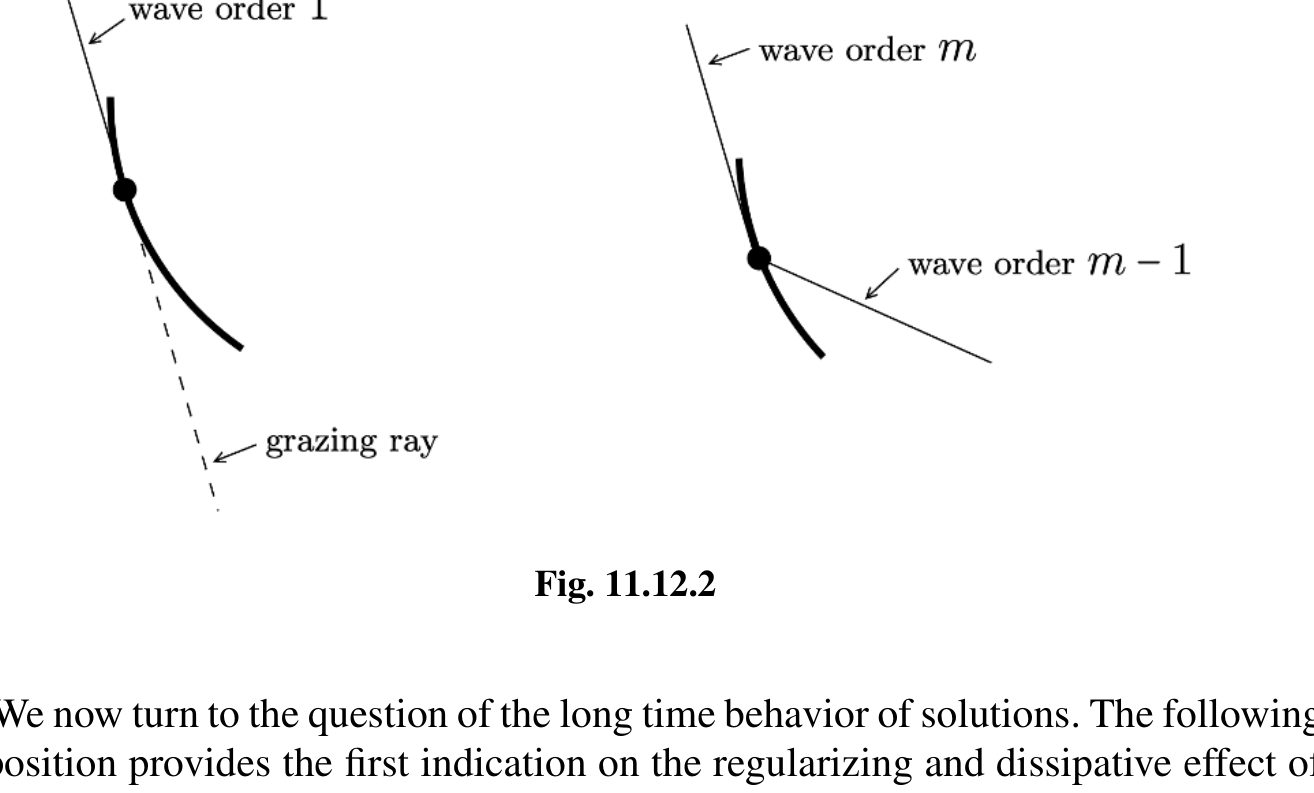
\includegraphics[width=0.75\textwidth]{ch11-fig12-2.png}
\caption{弱波的产生: 1 阶弱波由掠射线触发; $m$ 阶弱波由 $m-1$ 阶弱波与左接触间断碰撞产生。}
\label{figure:ch11-11-12-2}
\end{figure}

现转向解的长时间行为问题。如下命题给出通量 $f$ 非线性的正则化与耗散效应的初步指示。

\begin{theorem}\label{theorem:ch11-11-12-3}
设 $u$ 是\eqref{align:ch11-11-12-1} Cauchy 问题的可容许 $BV$ 解, 初值 $u_0\in L^1(-\infty,\infty)$。则
\begin{align}
TV_{(-\infty,\infty)}F(u(\cdot,t))\leqslant\frac{2}{t}\int_{-\infty}^\infty|u_0(x)|\,dx,\qquad 0<t<\infty,\label{align:ch11-11-12-20}
\end{align}
其中 $F$ 是单调递增函数
\begin{align}
F(u)=f(u)-uf'(u),\qquad -\infty<u<\infty.\label{align:ch11-11-12-21}
\end{align}
\end{theorem}

\begin{proof}
固定 $t>0$, 取任意网格 $-\infty<x_{-\ell}<\cdots<x_0<\cdots<x_s<\infty$, 使 $u(x_i+,t)=u(x_i,t)$, $i=-\ell,\ldots,s$, 且当 $i$ 偶时 $u(x_i,t)<u(x_{i+1},t)$, 当 $i$ 奇时 $u(x_i,t)>u(x_{i+1},t)$。

对每个 $i=-\ell,\ldots,s$, 关联一条从点 $(x_i,t)$ 出发的后向特征线 $\chi_i(\cdot)$, 它在 $(0,t)$ 上是左接触, 确定如下:

(a) 当 $i$ 偶且 $u(x_i,t)<0$, 或当 $i$ 奇且 $u(x_i,t)>0$ 时, $\chi_i(\cdot)$ 是从 $(x_i,t)$ 出发的极小后向特征线 $\phi_i(\cdot)$。

(b) 当 $i$ 偶且 $u(x_i,t)>0$, 或当 $i$ 奇且 $u(x_i,t)<0$ 时, $\chi_i(\cdot)$ 通过如下过程识别。考虑从 $(x_i,t)$ 出发的极大后向特征线 $\psi_i(\cdot)$, 由\cref{theorem:ch11-11-12-2}, 其图像是以点 $(\psi(a_n),a_n)$ 为顶点的多边形链, 其中 $0=a_0<a_1<\cdots<a_{k+1}=t$。若 $k=0$ 或 $k=1$, 在 $[0,t]$ 上识别 $\chi_i(\cdot)$ 为 $\psi_i(\cdot)$。相反, 若 $k\geqslant2$, 构造从点 $(\psi_i(a_{k-1}),a_{k-1})$ 出发的极小后向特征线 $\phi_i(\cdot)$, 在时间区间 $[a_{k-1},t]$ 上识别 $\chi_i(\cdot)$ 为 $\psi_i(\cdot)$, 在时间区间 $[0,a_{k-1}]$ 上识别为 $\phi(\cdot)$。

易见 $\chi_i(\cdot)$ 与 $\chi_{i+1}(\cdot)$ 的图像在 $(0,t]$ 上不相交。于是在集合 $\{(x,\tau):0<\tau<t,\ \chi_i(\tau)<x<\chi_{i+1}(\tau)\}$ 上积分\eqref{align:ch11-11-12-1}。由于 $\chi_i(\cdot)$ 与 $\chi_{i+1}(\cdot)$ 均为左接触, 回忆\eqref{align:ch11-11-12-21}推出
\begin{align}
\int_0^t F(u(\chi_{i+1}(\tau),\tau))\,d\tau-\int_0^t F(u(\chi_i(\tau),\tau))\,d\tau\nonumber\\
=\int_{\chi_i(0)}^{\chi_{i+1}(0)}u_0(x)\,dx-\int_{x_i}^{x_{i+1}}u(x,t)\,dx.\label{align:ch11-11-12-22}
\end{align}

现证
\begin{align}
\left|\int_0^t F(u(\chi_{i+1}(\tau),\tau))\,d\tau-\int_0^t F(u(\chi_i(\tau),\tau))\,d\tau\right|\nonumber\\
\geqslant t|F(u(x_{i+1},t))-F(u(x_i,t))|.\label{align:ch11-11-12-23}
\end{align}
为验证\eqref{align:ch11-11-12-23}, 须研究可能出现的不同情形, 取决于 $i$ 奇偶以及 $u(x_i,t)$ 与 $u(x_{i+1},t)$ 的符号。这里仅讨论两种代表性情形。

先设 $u(x_i,t)<0<u(x_{i+1},t)$(特别地, $i$ 偶)。此时 $\chi_i(\cdot)$ 与 $\chi_{i+1}(\cdot)$ 分别是从 $(x_i,t)$ 与 $(x_{i+1},t)$ 出发的极小后向特征线 $\phi_i(\cdot)$ 与 $\phi_{i+1}(\cdot)$。由\cref{theorem:ch11-11-12-2}, 对 $\tau\in(0,t)$, $u(\chi_i(\tau),\tau)\leqslant u(x_i,t)$ 且 $u(\chi_{i+1}(\tau),\tau)\geqslant u(x_{i+1},t)$。由于 $F$ 递增, 得\eqref{align:ch11-11-12-23}。

再设 $0<u(x_i,t)<u(x_{i+1},t)$(特别地, $i$ 偶)。此时 $\chi_{i+1}(\cdot)$ 仍是从 $(x_{i+1},t)$ 出发的极小后向特征线 $\phi_i(\cdot)$, 故如上 $u(\chi_{i+1}(\tau),\tau)\geqslant u(x_{i+1},t)$。另一方面, $\chi_i(\cdot)$ 在时间区间 $[a_{k-1},t]$ 上与从 $(x_i,t)$ 出发的极大后向特征线 $\psi_i(\cdot)$ 重合, 在时间区间 $[0,a_{k-1}]$ 上与从点 $(\psi_i(a_{k-1},a_{k-1}))$ 出发的极小后向特征线 $\phi(\cdot)$ 重合。现观察到 $u(\chi_i(\tau),\tau)=u(x_i,t)$ 对 $\tau\in[a_{k-1},t]$, 且 $u(\chi_i(\tau),\tau)\leqslant0$ 对 $\tau\in(0,a_k)$。于是此情形\eqref{align:ch11-11-12-23}亦成立。

一旦\eqref{align:ch11-11-12-23}建立, 与\eqref{align:ch11-11-12-22}合并并对 $i=-\ell,\ldots,s-1$ 求和。回忆\cref{chapter:ch06-标量守恒律L1理论}, 得\eqref{align:ch11-11-12-20}。证毕。

\end{proof}

初值局部有界变差的假设在推导估计\eqref{align:ch11-11-12-20}时未起作用。因此, 通过完备化可推出: 若 $u$ 是\eqref{align:ch11-11-12-1} Cauchy 问题的可容许解, 初值仅属于 $L^\infty(-\infty,\infty)$, 则对任意固定 $t>0$, 函数 $F(u(\cdot,t))$ 在 $(-\infty,\infty)$ 上局部有界变差。这特别蕴含单侧极限 $u(x\pm,t)$ 对所有 $(x,t)\in(-\infty,\infty)\times(0,\infty)$ 存在。于是可将广义特征线的概念与理论推广到此类解的范围。此外, 由\eqref{align:ch11-11-12-3}, $|v-w|^{m+1}\leqslant c|F(v)-F(w)|$, 故对任意固定 $t>0$, $u(\cdot,t)$ 属于分数阶 $\frac{1}{m+1}$ 有界变差函数空间。事实上, 如\cref{chapter:ch11-一维标量守恒律}所列参考文献所示, 对任意 $t\geqslant0$, 特征速度 $f'(u(\cdot,t))$ 在 $(-\infty,\infty)$ 上局部有界变差。因此 $u(\cdot,t)$ 属于分数阶 $\frac{1}{m}$ 局部有界变差函数空间。这是 present 情形下\cref{theorem:ch11-11-2-2}的对应物。


在着手下一个课题, 即研究初值为周期或紧支撑时解的长时间行为之前, 需要如下准备。

对任意 $u\neq0$, 关联唯一的 $u^*\neq u$, 满足
\begin{align}
f'(u)=\frac{f(u^*)-f(u)}{u^*-u}.\label{align:ch11-11-12-24}
\end{align}
于是 $u^*$ 是可在右侧以左接触间断与 $u$ 连接的唯一状态。已知 $u$ 与 $u^*$ 符号相反, 且 $f'(u^*)<f'(u)$。由\eqref{align:ch11-11-12-3}还可证
\begin{align}
\lim_{u\to0}\frac{f'(u)}{f'(u^*)}=\rho_m,\label{align:ch11-11-12-25}
\end{align}
其中 $\rho_m$ 是方程
\begin{align}
m\rho^{\frac{m+1}{m}}+(m+1)\rho-1=0\label{align:ch11-11-12-26}
\end{align}
的唯一正解。例如 $m=2$ 时 $\rho_2=\frac14$。应注意 $\rho_m<\frac{1}{m+1}$。

先从紧支撑初值情形开始。

\begin{theorem}\label{theorem:ch11-11-12-4}
设 $u$ 是\eqref{align:ch11-11-12-1} Cauchy 问题的可容许 $BV$ 解, 初值 $u_0$ 支撑于区间 $[-\ell,0]$ 并携带质量
\begin{align}
\int_{-\ell}^0 u_0(x)\,dx=M.\label{align:ch11-11-12-27}
\end{align}
则当 $t\to\infty$,
\begin{align}
f'(u(x,t))=
\begin{cases}
0, & -\infty<x\leqslant\chi(t)\\
\dfrac{x}{t}+O(t^{r-1}), & \chi(t)<x\leqslant0\\
0, & 0<x<\infty,
\end{cases}\label{align:ch11-11-12-28}
\end{align}
其中 $r$ 是满足 $\rho_m<r<\frac{1}{m+1}$ 的任意常数, 且
\begin{align}
\chi(t)=-\left[\frac{m+1}{m}|M|\right]^{\frac{m}{m+1}}t^{\frac{1}{m+1}}+O(t^r).\label{align:ch11-11-12-29}
\end{align}
\end{theorem}

\begin{proof}
显然, $x=0$ 是从 $(0,0)$ 出发的极大前向特征线, 故对任意 $x>0$, $u(x,t)=0$。类似地, 设 $\chi(\cdot)$ 是从 $(-\ell,0)$ 出发的极小前向特征线, 则对所有 $x<\chi(t)$, $u(x,t)=0$。

固定任意 $r\in(\rho_m,\frac{1}{m+1})$。由\eqref{align:ch11-11-12-25}, 存在 $\delta>0$ 使
\begin{align}
f'(u)>r f'(u^*),\qquad -\delta\leqslant u\leqslant\delta.\label{align:ch11-11-12-30}
\end{align}
由\cref{theorem:ch11-11-12-3}与\eqref{align:ch11-11-12-3}, $u(x,t)=O(t^{-\frac{1}{m+1}})$, $t\to\infty$, 对 $x$ 一致。故存在 $T>0$ 使 $|u(x,t)|\leqslant\delta$, 对 $-\infty<x<\infty$, $t\geqslant T$。

现固定任意点 $(x,t)$, $t>T$, $\chi(t)<x<0$ 且 $u(x+,t)=u(x,t)\neq0$, 验证\eqref{align:ch11-11-12-28}。考虑从 $(x,t)$ 出发的极小后向特征线 $\phi(\cdot)$, 性质见\cref{theorem:ch11-11-12-1}。由于 $\phi(\cdot)$ 凸, $x-tf'(u(x,t))\leqslant\phi(0)\leqslant0$, 这给出\eqref{align:ch11-11-12-28}中断言的 $f'(u(x,t))$ 的上界。下界由如下过程推导。

识别 $\phi(\cdot)$ 被时间线 $t=T$ 截获的点 $\phi(T)$。当 $\phi(\cdot)$ 在 $(T,t)$ 上无激波时, 立即得到 $f'(u(x,t))$ 的期望下界, 因为此情形下
\begin{align}
x-tf'(u(x,t))=\phi(T)-Tf'(u(x,t))\geqslant\phi(T)\geqslant-\ell-\lambda T,\label{align:ch11-11-12-31}
\end{align}
其中 $\lambda$ 是 $-f'$ 在 $[-\bar u,\bar u]$ 上的任意上界。

另一种更困难情形出现于 $\phi(\cdot)$ 在时间区间 $(\alpha,t)$, $\alpha\in(T,t)$ 上无激波, 但 $u(\phi(\alpha)+,\alpha)\neq u(\phi(\alpha),\alpha)$。此情形下
\begin{align}
x-tf'(u(x,t))=\phi(\alpha)-\alpha f'(u(x,t))\geqslant\phi(\alpha),\label{align:ch11-11-12-32}
\end{align}
故需 $\phi(\alpha)$ 的下界。为此, 证 $\phi(\cdot)$ 满足微分不等式
\begin{align}
\dot{\phi}(\tau)\geqslant\frac{r}{\tau}\phi(\tau),\qquad T\leqslant\tau\leqslant\alpha.\label{align:ch11-11-12-33}
\end{align}

先对任意 $\tau$ 且 $u(\phi(\tau)+,\tau)\neq u(\phi(\tau),\tau)$ 验证\eqref{align:ch11-11-12-33}。设 $\psi(\cdot)$ 是从点 $(\phi(\tau),\tau)$ 出发的极大后向特征线。由\cref{theorem:ch11-11-12-2}与\eqref{align:ch11-11-12-30}, 回忆 $|u(\phi(\tau),\tau)|\leqslant\delta$,
\begin{align}
\dot{\phi}(\tau)=f'(u(\phi(\tau),\tau))\geqslant r f'(u(\phi(\tau)+,\tau))=r\dot{\psi}(\tau)\geqslant r\dot{\psi}(s),\label{align:ch11-11-12-34}
\end{align}
对 $s\in[0,\tau]$。在 $[0,\tau]$ 上关于 $s$ 积分\eqref{align:ch11-11-12-34}, 回忆 $\psi(0)\leqslant0$, $\psi(\tau)=\phi(\tau)$, 推出
\begin{align}
\tau\dot{\phi}(\tau)\geqslant r\phi(\tau),\label{align:ch11-11-12-35}
\end{align}
这对此类 $\tau$ 建立了\eqref{align:ch11-11-12-33}。

接下来考虑任意 $\tau\in[T,\alpha]$ 且 $u(\phi(\tau)+,\tau)=u(\phi(\tau),\tau)$。此情形下, 由\cref{theorem:ch11-11-12-1}, 存在 $\beta\in(\tau,\alpha]$ 使 $\phi(\cdot)$ 在 $[\tau,\beta)$ 上无激波但 $u(\phi(\beta)+,\beta)\neq u(\phi(\beta),\beta)$。特别地,
\begin{align}
\phi(\beta)-\beta\dot{\phi}(\beta)=\phi(\tau)-\tau\dot{\phi}(\beta)\label{align:ch11-11-12-36}
\end{align}
且 $\dot{\phi}(\tau)=\dot{\phi}(\beta)$。此外, 如上所示 $\beta\dot{\phi}(\beta)\geqslant r\phi(\beta)$。于是
\begin{align}
r\phi(\tau)-\tau\dot{\phi}(\tau)=r\phi(\beta)-\beta\dot{\phi}(\beta)+(1-r)(\beta-\tau)\dot{\phi}(\beta)\leqslant0,\label{align:ch11-11-12-37}
\end{align}
这对此类 $\tau$ 也建立了\eqref{align:ch11-11-12-33}。

积分微分不等式\eqref{align:ch11-11-12-33}, 断定 $\phi(\alpha)$ 是 $O(\alpha^r)$, 从而更有 $O(t^r)$。连同\eqref{align:ch11-11-12-32}完成\eqref{align:ch11-11-12-28}的证明。

最后, 由质量守恒确定 $\chi(t)$:
\begin{align}
\int_{\chi(t)}^0 u(x,t)\,dx=\int_{-\ell}^0 u_0(x)\,dx=M.\label{align:ch11-11-12-38}
\end{align}
注意\eqref{align:ch11-11-12-28}允许两个值:
\begin{align}
u(x,t)=\pm\left[-\frac{x}{t}\right]^{\frac{1}{m}}+O\left(t^{r-\frac{2}{m+1}}\right).\label{align:ch11-11-12-39}
\end{align}
然而, 激波可容许性排除从 $(-x/t)^{1/m}$ 到 $-(-x/t)^{1/m}$ 或反向的跳跃, 故 $u$ 在 $(\chi(t),0)$ 上保持恒定符号, 即当 $M>0$ 为正, 当 $M<0$ 为负。两种情形下, 合并\eqref{align:ch11-11-12-39}与\eqref{align:ch11-11-12-38}, 得\eqref{align:ch11-11-12-29}。证毕。
\end{proof}

以周期情形的讨论结束本节。

\begin{theorem}\label{theorem:ch11-11-12-5}
设 $u$ 是\eqref{align:ch11-11-12-1} Cauchy 问题的可容许 $BV$ 解, 初值 $u_0$ 周期:
\begin{align}
u_0(x+\ell)=u_0(x),\qquad -\infty<x<\infty,\label{align:ch11-11-12-40}
\end{align}
且零均值
\begin{align}
\int_0^\ell u_0(x)\,dx=0.\label{align:ch11-11-12-41}
\end{align}
则
\begin{align}
-f'(u(x,t))\leqslant\frac{k\ell}{t},\qquad -\infty<x<\infty,\ 0<t<\infty.\label{align:ch11-11-12-42}
\end{align}
\end{theorem}

\begin{proof}
回忆由\eqref{align:ch11-11-12-24}构造的 $u^*$ 的\eqref{align:ch11-11-12-25}, 推出存在 $\rho<1$ 使
\begin{align}
f'(u)>\rho f'(u^*),\qquad -\bar u\leqslant u\leqslant\bar u.\label{align:ch11-11-12-43}
\end{align}
我们证明, 对每个使 $u(y,t)$ 与 $u(y+,t)$ 异号的 $(y,t)$,
\begin{align}
-t f'(u(y+,t))\leqslant\hat{k}\ell,\label{align:ch11-11-12-44}
\end{align}
其中常数 $\hat{k}$ 仅依赖于 $\rho$。

考虑从 $(y,t)$ 出发的极大后向特征线 $\psi(\cdot)$。由\cref{theorem:ch11-11-12-2}, $\psi(\cdot)$ 的图像是以点 $(\psi(a_n),a_n)$ 为顶点的多边形链, 其中 $0=a_0<a_1<\cdots<a_{k+1}=t$。对固定 $n=1,\ldots,k+1$, 设 $\phi_n(\cdot)$ 表示从链顶点 $(\psi(a_n),a_n)$ 出发的极小后向特征线。要点是证
\begin{align}
\dot{\phi}_n(\tau)\geqslant\rho\frac{a_n-a_{n-1}}{\tau-a_{n-1}}f'(u(\psi(a_n)+,a_n)),\qquad \tau\in(a_{n-1},a_n].\label{align:ch11-11-12-45}
\end{align}

先对任意 $\tau\in(a_{n-1},a_n]$ 且 $u(\phi_n(\tau)+,\tau)\neq u(\phi_n(\tau),\tau)$ 验证\eqref{align:ch11-11-12-45}。设 $\chi(\cdot)$ 是从点 $(\phi_n(\tau),\tau)$ 出发的极大后向特征线。于是, 由\cref{theorem:ch11-11-11-1}与\cref{theorem:ch11-11-11-2}, 回忆\eqref{align:ch11-11-12-43},
\begin{align}
\dot{\phi}_n(\tau)=f'(u(\phi_n(\tau),\tau))\geqslant\rho f'(u(\phi_n(\tau)+,\tau))=\rho\dot{\chi}(\tau)\geqslant\rho\dot{\chi}(s),\label{align:ch11-11-12-46}
\end{align}
对任意 $s\in[a_{n-1},\tau]$, 于是
\begin{align}
(\tau-a_{n-1})\dot{\psi}(\tau)\geqslant\rho\chi(\tau)-\rho\chi(a_{n-1}).\label{align:ch11-11-12-47}
\end{align}
合并\eqref{align:ch11-11-12-47}与
\begin{align}
\chi(a_{n-1})\leqslant\psi(a_{n-1})=\psi(a_n)-(a_n-a_{n-1})f'(u(\psi(a_n)+,a_n))\label{align:ch11-11-12-48}
\end{align}
且因 $\chi(\tau)-\phi_n(\tau)\geqslant\phi_n(a_n)=\psi(a_n)$, 得\eqref{align:ch11-11-12-45}。

接下来考虑任意 $\tau\in(a_{n-1},a_n)$ 且 $u(\phi_n(\tau)+,\tau)=u(\phi_n(\tau),\tau)$。由\cref{theorem:ch11-11-11-2}, 存在 $\beta\in(\tau,a_n]$ 使 $\phi_n(\cdot)$ 在 $[\tau,\beta)$ 上无激波, 但 $u(\phi_n(\beta)+,\beta)\neq u(\phi_n(\beta),\beta)$。如上, \eqref{align:ch11-11-12-45}对 $\tau=\beta$ 成立, 故
\begin{align}
\dot{\phi}_n(\tau)=\dot{\phi}_n(\beta)\geqslant\rho\frac{a_n-a_{n-1}}{\beta-a_{n-1}}f'(u(\psi(a_n)+,a_n))\nonumber\\
\geqslant\rho\frac{a_n-a_{n-1}}{\tau-a_{n-1}}f'(u(\psi(a_n)+,a_n)),\label{align:ch11-11-12-49}
\end{align}
这对此类 $\tau$ 也验证了\eqref{align:ch11-11-12-45}。

积分\eqref{align:ch11-11-12-45}, 得对任意 $\tau\in(a_{n-1},a_n)$,
\begin{align}
\phi_n(a_n)-\phi_n(\tau)\geqslant\rho(a_n-a_{n-1})\log\frac{a_n-a_{n-1}}{\tau-a_{n-1}}f'(u(\psi(a_n)+,a_n)).\label{align:ch11-11-12-50}
\end{align}
同时有
\begin{align}
\psi(\tau)-\psi(a_n)=-(a_n-\tau)f'(u(\psi(a_n)+,a_n)).\label{align:ch11-11-12-51}
\end{align}
相加\eqref{align:ch11-11-12-50}与\eqref{align:ch11-11-12-51}, 回忆 $\phi_n(a_n)=\psi(a_n)$。并注意 $\psi(\tau)-\phi_n(\tau)<\ell$, 否则从 $(\phi(a_n)-\ell,a_n)$ 出发的极大后向特征线将在区间 $(a_{n-1},a_n)$ 上与 $\phi_n(\cdot)$ 相交。于是取 $\tau=a_{n-1}+\rho(a_n-a_{n-1})$, 得
\begin{align}
-(a_n-a_{n-1})f'(u(\psi(a_n)+,a_n))\leqslant(1-\rho-\rho\log\rho)^{-1}\ell.\label{align:ch11-11-12-52}
\end{align}
由\eqref{align:ch11-11-12-12}、\eqref{align:ch11-11-12-25}与\eqref{align:ch11-11-12-43},
\begin{align}
\rho^{k+1-n}f'(u(\psi(a_n)+,a_n))\leqslant f'(u(y+,t)),\label{align:ch11-11-12-53}
\end{align}
故\eqref{align:ch11-11-12-52}给出
\begin{align}
-(a_n-a_{n-1})f'(u(y+,t))\leqslant\rho^{k+1-n}(1-\rho+\rho\log\rho)^{-1}\ell.\label{align:ch11-11-12-54}
\end{align}
对 $n=1,\ldots,k+1$ 求和\eqref{align:ch11-11-12-54}, 得\eqref{align:ch11-11-12-44}, 常数 $\hat{k}=[(1-\rho)(1-\rho+\rho\log\rho)]^{-1}$。

现证\eqref{align:ch11-11-12-42}。固定 $(x,t)$, $-\infty<x<\infty$, $t>0$。因 $u(\cdot,t)$ 零均值, 存在 $y\in[x-\ell,x]$ 使 $u(y,t)\leqslant0$, $u(y+,t)\geqslant0$。设 $\chi(\cdot)$ 与 $\psi(\cdot)$ 分别是从 $(x,t)$ 与 $(y,t)$ 出发的极大后向特征线。对 $\tau\in[t/2,t]$, $\dot{\chi}(\tau)\leqslant f'(u(x,t))$。此外, 用\eqref{align:ch11-11-12-44}, $-\tau\dot{\psi}(\tau)\leqslant2\hat{k}\ell$, $\tau\in[t/2,t]$。于是
\begin{align}
\chi\left(\frac{t}{2}\right)\geqslant x-\frac{t}{2}f'(u(x,t)),\label{align:ch11-11-12-55}
\end{align}
\begin{align}
\psi\left(\frac{t}{2}\right)\leqslant y+\hat{k}\ell.\label{align:ch11-11-12-56}
\end{align}
从\eqref{align:ch11-11-12-55}减去\eqref{align:ch11-11-12-56}, 并用 $x>y$ 与 $\chi(t/2)-\psi(t/2)\leqslant\ell$, 得\eqref{align:ch11-11-12-42}, $k=2(\hat{k}+1)$。证毕。
\end{proof}

\end{document}
